% Copyright 2026 Sreeram Anil
% SPDX-License-Identifier: CC-BY-4.0
\chapter{Gaussian-sum filter (GSF)}
\label{ch:gsf}

\section*{At a glance}
\begin{tabular}{@{}l>{\raggedright\arraybackslash}p{0.76\textwidth}@{}}
Family & Sequential Monte Carlo (particle / ensemble / Gaussian sum) \\
Header & \texttt{include/estkit/particle/gsf.hpp} \\
Registered name & \texttt{GSF} ($N_c = 3$ EKF components, spread along the SOC axis) \\
State dimension & $n_x = 4$ (cell model) — generic in $n_x, n_u, n_y$ \\
Cost per step & \SI{1.75}{\micro\second}/step ($3.7\times$ EKF; $N_c$ EKF cycles $+\mathcal{O}(N_c^2n_x^2)$) \\
Memory & \SI{9.2}{\kilo\byte} ($N_c$ means and covariances, one EKF workspace) \\
Primary references & \cite{alspach1972gsf,sorenson1971gsum,salmond1990mixture,andersonmoore1979} \\
\end{tabular}

\section{Motivation and aerospace/BMS relevance}
Between "one Gaussian" and "five hundred samples" there is a great deal of room.  A Gaussian
\emph{mixture} with a handful of components can represent skew, multi-modality and heavy tails far
better than a single Gaussian, while still propagating each component with the machinery --- and the
cost --- of a Kalman filter.  Alspach and Sorenson \cite{alspach1972gsf,sorenson1971gsum} showed
that any density can be approximated arbitrarily well in $L_1$ by a finite Gaussian sum, and that
the Bayesian recursion maps a Gaussian sum to a Gaussian sum exactly when the model is linear ---
and approximately, component by component, when it is not.

The practical argument for a battery is specific.  A single EKF linearises $\ocv(\soc)$ once, at
the current SOC estimate.  When the prior is broad --- an unknown initial SOC after a pack swap, a
wake-up from deep sleep, a re-initialisation after a sensor fault --- that single linearisation is
taken at a point that may be far from the truth, on a curve whose slope varies by a factor of three
across the usable SOC range.  A mixture spread along the SOC axis carries several linearisations at
once and lets the measurement likelihood decide between them.  This is the same idea as the
multiple-model estimators (IMM, MMAE) applied to a continuous parameter rather than to a discrete
mode.

The GSF is also the cheapest non-trivial method in this family by a wide margin:
\SI{1.75}{\micro\second}/step, only \num{3.7} times an EKF, which is what makes it the one
mixture-based method that could actually run on every cell of a pack.

\section{Problem statement and assumptions}
Model \eqref{eq:pfb-dyn}--\eqref{eq:pfb-meas}, with
\begin{quote}
(A8) $f$ and $h$ are well approximated by their first-order Taylor expansions over the support of
\emph{each individual component} (not over the support of the whole mixture), and the Jacobians
$\mF$, $\mH$ exist.
\end{quote}
(A8) is the assumption the whole method rests on: the mixture is useful precisely because its
components are narrow enough for (A8) to hold when the same assumption fails for a single Gaussian
covering the same prior.

\section{Derivation}

\subsection{Gaussian sums}
Approximate the filtering density by
\begin{equation}
  p(\vx_k\mid\vy_{1:k}) \;\approx\; \sum_{j=1}^{N_c} \alpha_j^{(k)}\; \N{\bm\mu_j^{(k)}}{\mP_j^{(k)}},
  \qquad \alpha_j \ge 0, \quad \textstyle\sum_j\alpha_j = 1 .
  \label{eq:gsf-mixture}
\end{equation}
Alspach and Sorenson's Lemma~1 \cite{alspach1972gsf} guarantees that the class of such sums is dense
in $L_1$, so \eqref{eq:gsf-mixture} is not a restriction in principle, only a question of how many
components one can afford.

\subsection{Time update}
Since the Chapman--Kolmogorov integral \eqref{eq:pfb-chapman} is linear in the density, it acts on
each component separately.  Under (A8) each component is propagated by an EKF time update:
\begin{equation}
  \bm\mu_j^- = f(\bm\mu_j^+,\vu_{k-1}), \qquad
  \mP_j^- = \mF_j\,\mP_j^+\,\mF_j^\T + \mQ, \qquad
  \mF_j = \left.\frac{\partial f}{\partial\vx}\right|_{\bm\mu_j^+},
  \label{eq:gsf-time}
\end{equation}
and the weights are unchanged, $\alpha_j^- = \alpha_j^+$.

\subsection{Measurement update and the weight recursion}
Bayes' rule \eqref{eq:pfb-bayes} applied to \eqref{eq:gsf-mixture} gives
\begin{equation}
  p(\vx_k\mid\vy_{1:k}) \;\propto\; p(\vy_k\mid\vx_k)\sum_j \alpha_j^- \N{\bm\mu_j^-}{\mP_j^-}
  \;=\; \sum_j \alpha_j^-\; \underbrace{p(\vy_k\mid\vx_k)\,\N{\bm\mu_j^-}{\mP_j^-}}_{\text{one component}} .
  \label{eq:gsf-bayes}
\end{equation}
For each component, the product of the Gaussian prior with the (linearised) Gaussian likelihood is,
up to a constant, again a Gaussian --- the Kalman posterior --- and the constant is the
\emph{predictive likelihood} of that component:
\begin{equation}
  \int p(\vy_k\mid\vx)\,\N{\bm\mu_j^-}{\mP_j^-}\,d\vx \;=\; \N{\bm e_j}{\mS_j},
  \qquad
  \bm e_j = \vy_k - h(\bm\mu_j^-,\vu_k), \quad \mS_j = \mH_j\mP_j^-\mH_j^\T + \mR .
  \label{eq:gsf-predlik}
\end{equation}
Hence the mixture update is
\begin{equation}
  \boxed{\;
  \alpha_j^+ = \frac{\alpha_j^-\, \N{\bm e_j}{\mS_j}}{\sum_{m}\alpha_m^-\,\N{\bm e_m}{\mS_m}},
  \qquad
  \bm\mu_j^+ = \bm\mu_j^- + \mK_j\bm e_j, \qquad
  \mP_j^+ = (\mI-\mK_j\mH_j)\mP_j^-(\cdot)^\T + \mK_j\mR\mK_j^\T \;}
  \label{eq:gsf-update}
\end{equation}
with $\mK_j = \mP_j^-\mH_j^\T\mS_j\inv$ \cite[eq.~(17)]{alspach1972gsf}.  Each component runs an
ordinary (Joseph-stabilised) EKF; the \emph{only} coupling between components is the normalisation
of the weights.  A component whose predicted voltage does not match the measurement loses weight
exponentially fast --- this is the hypothesis test that a single EKF cannot perform.

\subsection{Reported moments}
The estimate and its covariance are the mixture moments
\begin{equation}
  \xhat_k = \sum_j \alpha_j^+\bm\mu_j^+, \qquad
  \mP_k = \sum_j \alpha_j^+\Big[\mP_j^+ + (\bm\mu_j^+-\xhat_k)(\bm\mu_j^+-\xhat_k)^\T\Big].
  \label{eq:gsf-moments}
\end{equation}
The second term is the spread \emph{between} components and is what makes the reported
\code{soc\_std} larger than any single component's, correctly reflecting the ambiguity.

\subsection{Initialisation: splitting the prior}
The benchmark hands the filter one Gaussian $\N{\vx_0}{\mP_0}$.  It is split along a chosen
coordinate $j^\star$ (the SOC axis for the cell model) into $N_c$ equally weighted components,
\begin{equation}
  \bm\mu_m = \vx_0 + \delta_m\sqrt{(\mP_0)_{j^\star j^\star}}\;\bm e_{j^\star},
  \qquad
  \delta_m = \delta\left(\frac{2m}{N_c-1}-1\right),\quad m = 0,\dots,N_c-1,
  \qquad \alpha_m = \frac{1}{N_c},
  \label{eq:gsf-split-means}
\end{equation}
so for $N_c = 3$ the means are $\vx_0 + \{-\delta,0,+\delta\}\sigma_{\soc_0}\bm e_{\soc}$.  The
component covariances are shrunk so that the mixture reproduces $\mP_0$ exactly,
\begin{equation}
  (\mP_m)_{j^\star j^\star} = (\mP_0)_{j^\star j^\star}\,(1 - v), \qquad
  v = \frac{1}{N_c}\sum_m \delta_m^2
  \;\;\Big(= \tfrac23\delta^2 \text{ for } N_c=3\Big),
  \label{eq:gsf-split-cov}
\end{equation}
all other entries unchanged.  With $\delta = 1$, $N_c = 3$ this gives
$(\mP_m)_{\soc\soc} = \frac13(\mP_0)_{\soc\soc}$: three narrow components covering the same prior
uncertainty, each satisfying (A8) three times better than the original.  The factor $1-v$ is floored
at \num{0.05}, which is what happens for $\delta \ge \sqrt{3/2}$; beyond that point the split
inflates the prior instead of reproducing it, a behaviour the sensitivity study below exploits.

\subsection{Mixture reduction (Salmond's criterion)}
Left alone, components either converge to each other (redundant) or lose all their weight (dead).
Salmond \cite{salmond1990mixture} measures the cost of merging components $i$ and $j$ by the
increase in within-cluster scatter they cause,
\begin{equation}
  D_{ij} = \frac{\alpha_i\alpha_j}{\alpha_i+\alpha_j}\,
           (\bm\mu_i-\bm\mu_j)^\T\,\bar{\mP}^{-1}\,(\bm\mu_i-\bm\mu_j),
  \label{eq:gsf-salmond}
\end{equation}
with $\bar{\mP}$ the covariance of the whole mixture \eqref{eq:gsf-moments}; the cheapest pair is
merged, moment-preservingly,
\begin{equation}
  \alpha = \alpha_i+\alpha_j,\quad
  \bm\mu = \frac{\alpha_i\bm\mu_i + \alpha_j\bm\mu_j}{\alpha},\quad
  \mP = \sum_{m\in\{i,j\}}\frac{\alpha_m}{\alpha}\Big[\mP_m + (\bm\mu_m-\bm\mu)(\bm\mu_m-\bm\mu)^\T\Big].
  \label{eq:gsf-merge}
\end{equation}
Because the bank has a compile-time size, the freed slot is refilled by splitting the heaviest
component; the split distance \code{split\_delta} controls whether this is an exact duplication
($\delta_s=0$) or a genuine re-spread.  Both merging and re-splitting are \emph{disabled by
default}, for reasons the next section quantifies.

\section{Algorithm}
\begin{algorithm}[H]
\caption{GSF --- one sampling period}
\begin{algorithmic}[1]
\Require components $\{\alpha_j,\bm\mu_j,\mP_j\}_{j=1}^{N_c}$, $\vu_{k-1},\vu_k,\vy_k$
\For{$j=1$ \textbf{to} $N_c$} \Comment{time update, one EKF each}
  \State $\bm\mu_j \gets f(\bm\mu_j,\vu_{k-1})$; \quad $\mP_j \gets \mF_j\mP_j\mF_j^\T + \mQ$
\EndFor
\State \textbf{Prior predictive.} $\yhat_k \gets \sum_j \alpha_j\, h(\bm\mu_j,\vu_k)$
\For{$j=1$ \textbf{to} $N_c$} \Comment{measurement update}
  \State $\bm e_j \gets \vy_k - h(\bm\mu_j,\vu_k)$; \quad $\mS_j \gets \mH_j\mP_j\mH_j^\T+\mR$; \quad $\mK_j \gets \mP_j\mH_j^\T\mS_j\inv$
  \State $\log\tilde\alpha_j \gets \log\alpha_j + \log\N{\bm e_j}{\mS_j}$
  \State $\bm\mu_j \gets \operatorname{constrain}(\bm\mu_j + \mK_j\bm e_j)$; \quad $\mP_j \gets$ Joseph form
\EndFor
\State $\alpha_j \gets \tilde\alpha_j/\sum_m\tilde\alpha_m$ (computed with the max-shift in the log domain)
\If{\code{reduce}} \State Salmond merge \eqref{eq:gsf-salmond}--\eqref{eq:gsf-merge} of the cheapest pair, then re-split the heaviest \EndIf
\State $\xhat_k,\ \mP_k$ from \eqref{eq:gsf-moments}
\Ensure $\xhat_k$, $\mP_k$, updated mixture
\end{algorithmic}
\end{algorithm}

\noindent One \code{Ekf<Model>} object is used as a workspace for all $N_c$ components (it is a pure
function of $(\vx,\mP)$ between calls), so only $N_c$ means and covariances are stored and the model
--- whose OCV table dominates its size --- is held once.

\section{Application to the battery model}
The spread coordinate is \code{EcmModel::IZ}, set in the registration lambda; the filter itself
never assumes which state that is.  Note that the largest prior variance in $\mP_0$ belongs to the
\emph{hysteresis} state ($\sigma_h = 0.5$ against $\sigma_{\soc} = 0.1$), so an automatic "split
along the most uncertain coordinate" rule would split the wrong axis --- the choice has to come from
the application, which is why it is an \code{Options} field rather than a heuristic.

\paragraph{Sensitivity to the spread $\delta$ (steady-state SOC RMSE in \%, development run,
seed 1; the EKF column is from the same run).}
\begin{center}
\begin{tabular}{@{}lccc|c@{}}
\toprule
 & $\delta = 0.5$ & $\delta = 1$ & $\delta = 2$ & EKF \\
\midrule
\code{nominal}         & 0.06 & 0.08 & 0.06 & 0.06 \\
\code{init\_error}     & 0.09 & 0.10 & 0.16$^\ddagger$ & 0.06 \\
\code{param\_mismatch} & 0.77 & 2.27 & 1.98 & 1.56 \\
\code{aged\_cell}      & 1.31 & 3.38 & 3.41 & 1.30 \\
\code{combined}        & 9.72$^\dagger$ & 3.89 & 2.43$^\ddagger$ & 12.22$^\dagger$ \\
\bottomrule
\end{tabular}
\end{center}
\noindent ($^\dagger$ never converges; $^\ddagger$ converges only after \SIrange{200}{400}{\second}.)
The non-monotonicity is real and worth understanding.  At $\delta = 0.5$ the components overlap
heavily ($0.5\sigma$ apart, each with $0.83\sigma^2$ of variance), the weights stay nearly uniform
and the filter is an EKF with a slightly conservative prior --- excellent when the model is right,
useless when the posterior is genuinely multi-modal (\code{combined} fails exactly as the EKF does).
At $\delta = 2$ the shrink floor in \eqref{eq:gsf-split-cov} binds, the mixture covariance is
$2.7\times$ the prior, and the extra prior spread is what rescues \code{combined} --- at the price of
narrow components that cannot move fast, hence the \SI{200}{\second} initial convergence.  The
shipped default $\delta = 1$ is the exact moment-matched split; it keeps the immediate initial-error
convergence and still improves \code{combined} by a factor \num{3.1} over the EKF.

\paragraph{Why merging is disabled by default.}
With the Salmond criterion active and a threshold of $D_{ij} < 0.1$, the three components of a
converged filter are merged at essentially every step, and the bank collapses to one component ---
mathematically correct (a converged posterior is unimodal) but it discards precisely the diversity
that rescues the biased scenarios.  Measured on the same development run: with \code{reduce = true} and $\delta = 1$,
\code{combined} degrades from \SI{3.89}{\percent} to \SI{12.20}{\percent} (i.e.\ back to EKF
behaviour), while \code{nominal} improves only from \SI{0.08}{\percent} to \SI{0.06}{\percent}.  The default is therefore
\code{reduce = false}; the machinery is retained and documented because for a bank that is allowed
to \emph{grow} (adaptive $N_c$) mixture reduction is mandatory.

\paragraph{Why re-splitting after a merge must be moment preserving.}
An early version re-spread the heaviest component by $\pm 0.7$ of its own standard deviation after
every merge.  Splitting a Gaussian into two displaced narrower Gaussians is \emph{not} an identity
on densities, so the subsequent measurement update collapses the weights onto one half and the
mixture covariance shrinks by a factor $1-\delta_s^2 = 0.51$ per step.  The covariance then falls
ten times below the EKF's, the filter becomes over-confident and locks in an early bias: measured
$\mathrm{RMSE}_{\mathrm{ss}} = \SI{4.7}{\percent}$ on \code{nominal}, i.e.\ sixty times worse than
the default.
\code{split\_delta} defaults to zero (exact duplication) and the episode is recorded here because
"split and let the data choose" is an intuitive and badly wrong idea.

\section{Implementation notes}
\emph{Cost and memory.}  \SI{1.75}{\micro\second}/step and \SI{9.2}{\kilo\byte}: three EKF cycles
(\SI{0.48}{\micro\second} each) plus the mixture moments and, when enabled, an $N_c\times N_c$
Salmond scan with one $n_x\times n_x$ inverse.  This is $44\times$ cheaper than \estname{PF-Bootstrap}
and $3.7\times$ an EKF, which makes it the only method in this family that is realistic for
per-cell deployment in a large pack.

\emph{Weight arithmetic.}  Weights are updated in the log domain with the max-shift normalisation of
\code{pf::normalize\_log\_weights}, and floored at $10^{-12}$ before the logarithm so that a
component which has been rejected for a long time can still be revived if the data change --- a
plain multiplicative update would underflow to exactly zero and never recover.

\emph{Component covariances.}  Each component uses the Joseph form, inherited from \code{Ekf}, and
\code{constrain()} is applied to each component mean, so every hypothesis stays physical.  $\mP_k$
is symmetrised after the mixture sum.

\emph{Determinism.}  The GSF is deterministic; \code{seed()} exists only for interface symmetry with
the rest of the family and does nothing.

\section{Benchmark results}
% Copyright 2026 Sreeram Anil
% SPDX-License-Identifier: CC-BY-4.0
\begin{table}[H]\centering\footnotesize\setlength{\tabcolsep}{4pt}
\caption{GSF: cell-level benchmark on the eVTOL mission (mean over seeds; RMSE and max error in \% SOC; $t_\mathrm{conv}$: first time the error stays below 2\,\% for 60\,s, -- = never; EKF reference: steady-state RMSE of the plain EKF on the same data).}\label{tab:cell_GSF}
\begin{tabular}{llrrrrrcrr}\toprule
plant & scenario & RMSE & RMSE$_\mathrm{ss}$ & max & $t_\mathrm{conv}$ [s] & RMSE$_v$ [mV] & div. & EKF ref. & ns/step \\ \midrule
ECM & nominal & 0.20 & 0.05 & 0.78 & 0 & 0.83 & no & 0.05 & 1749 \\
ECM & init\_error & 0.27 & 0.10 & 7.33 & 0 & 2.09 & no & 0.05 & 1743 \\
ECM & current\_bias & 0.48 & 0.55 & 1.06 & 0 & 0.89 & no & 0.61 & 1755 \\
ECM & noise\_step & 0.22 & 0.09 & 0.78 & 0 & 2.90 & no & 0.12 & 1753 \\
ECM & outliers & 1.07 & 0.12 & 10.20 & 57 & 2.07 & no & 0.21 & 1758 \\
ECM & cold & 0.22 & 0.15 & 0.79 & 0 & 1.91 & no & 0.16 & 1751 \\
ECM & hot & 0.16 & 0.03 & 0.73 & 0 & 0.59 & no & 0.03 & 1749 \\
ECM & aged\_cell & 4.67 & 3.12 & 21.67 & 0 & 3.32 & no & 1.52 & 1754 \\
ECM & param\_mismatch & 2.87 & 2.20 & 18.16 & 0 & 2.63 & no & 1.36 & 1773 \\
ECM & sensor\_dropout & 0.61 & 0.10 & 8.90 & 0 & 1.75 & no & 0.46 & 1755 \\
ECM & preisach & 0.87 & 0.20 & 4.45 & 94 & 0.89 & no & 0.20 & 1751 \\
ECM & combined & 5.34 & 3.33 & 29.36 & 0 & 4.16 & no & 12.44 & 1734 \\
\midrule
SPM & nominal & 2.21 & 1.39 & 5.77 & 0 & 1.05 & no & 3.73 & 1665 \\
SPM & init\_error & 4.17 & 3.99 & 8.15 & -- & 2.15 & no & 3.81 & 1662 \\
SPM & current\_bias & 3.55 & 3.86 & 7.54 & 0 & 1.15 & no & 5.69 & 1665 \\
SPM & noise\_step & 2.16 & 1.21 & 5.77 & 0 & 3.15 & no & 3.30 & 1669 \\
SPM & outliers & 3.15 & 1.25 & 10.20 & 217 & 2.29 & no & 1.99 & 1666 \\
SPM & cold & 5.66 & 5.14 & 10.78 & -- & 4.45 & no & 7.35 & 1672 \\
SPM & hot & 1.86 & 1.70 & 3.31 & 0 & 0.75 & no & 2.16 & 1654 \\
SPM & param\_mismatch & 3.11 & 3.50 & 14.90 & 0 & 1.92 & no & 3.13 & 1670 \\
SPM & sensor\_dropout & 2.84 & 1.85 & 9.63 & 0 & 1.96 & no & 5.31 & 1668 \\
\bottomrule\end{tabular}\end{table}

\begin{figure}[H]\centering
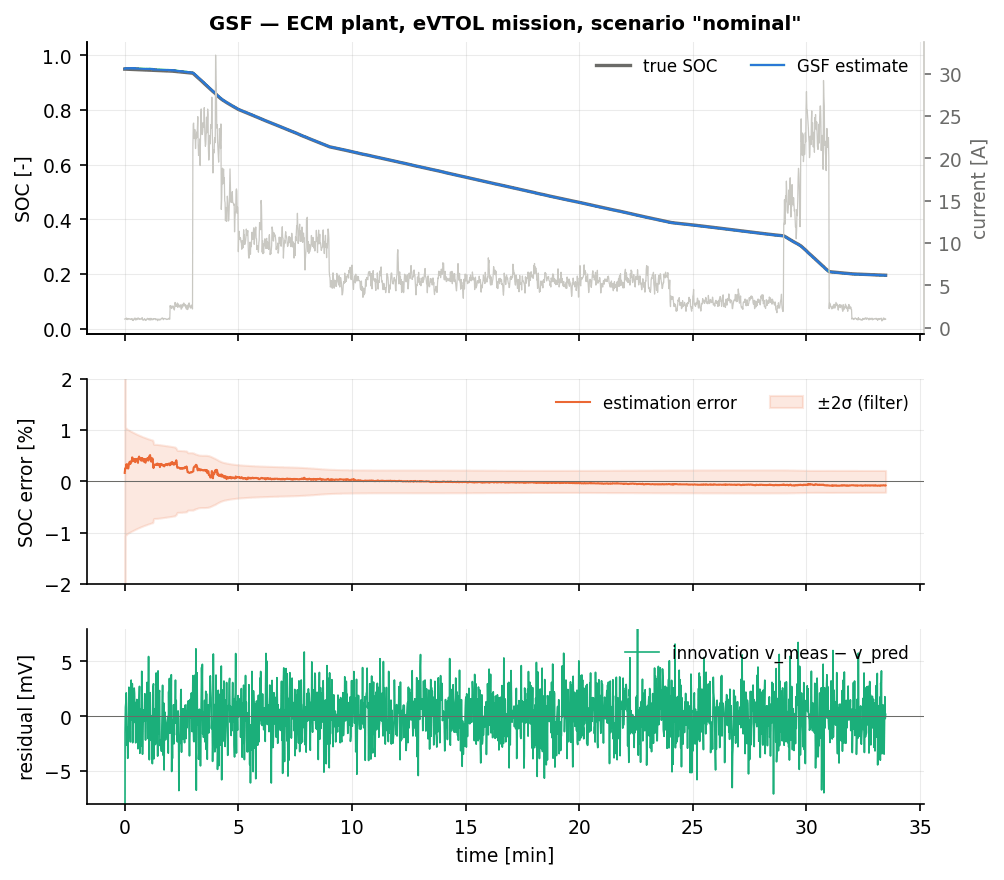
\includegraphics[width=\textwidth]{figures/cell_GSF_nominal.png}
\caption{GSF on the nominal eVTOL mission: true and estimated SOC (top), estimation error with the
$\pm2\sigma$ band from the mixture covariance \eqref{eq:gsf-moments} (middle), voltage residual
(bottom).}
\end{figure}
\begin{figure}[H]\centering
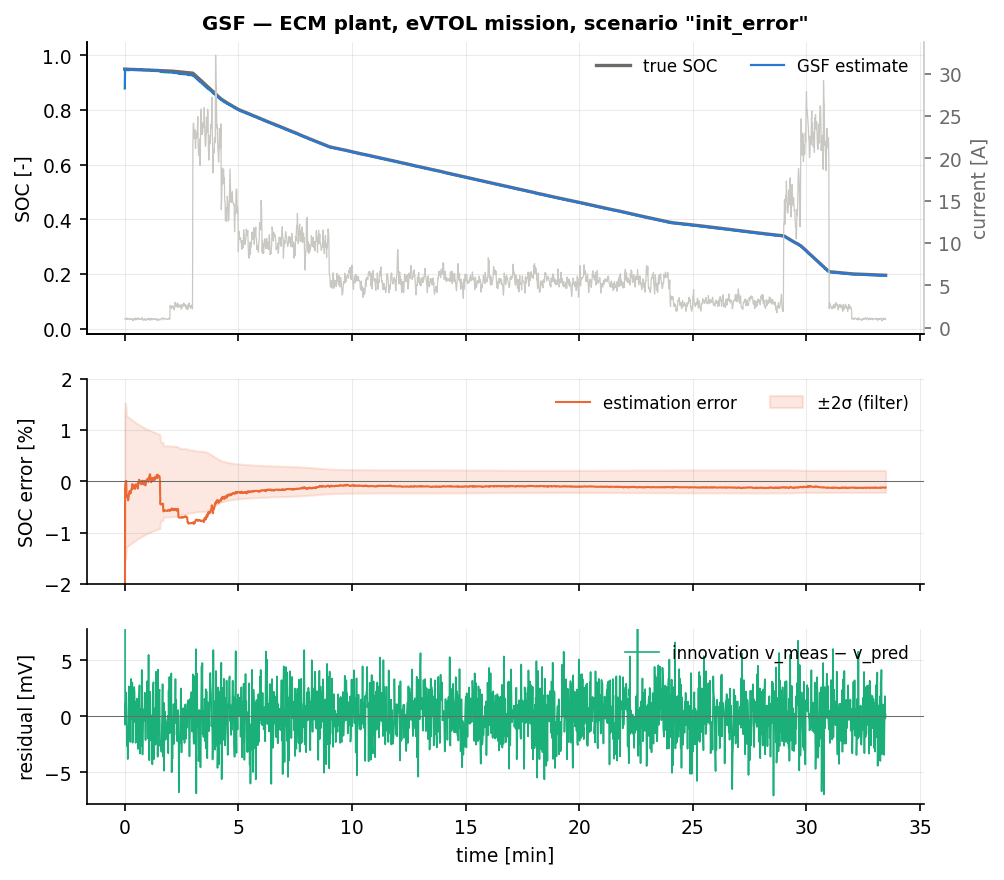
\includegraphics[width=\textwidth]{figures/cell_GSF_init_error.png}
\caption{GSF with a \SI{35}{\percent} initial SOC error --- the target scenario.  The three
components are initialised at $\soc_0 + \{-1,0,+1\}\sigma_{\soc_0}$; the weights concentrate on the
upper component within the first samples and the \SI{2}{\percent} band is reached immediately.}
\end{figure}
\begin{figure}[H]\centering
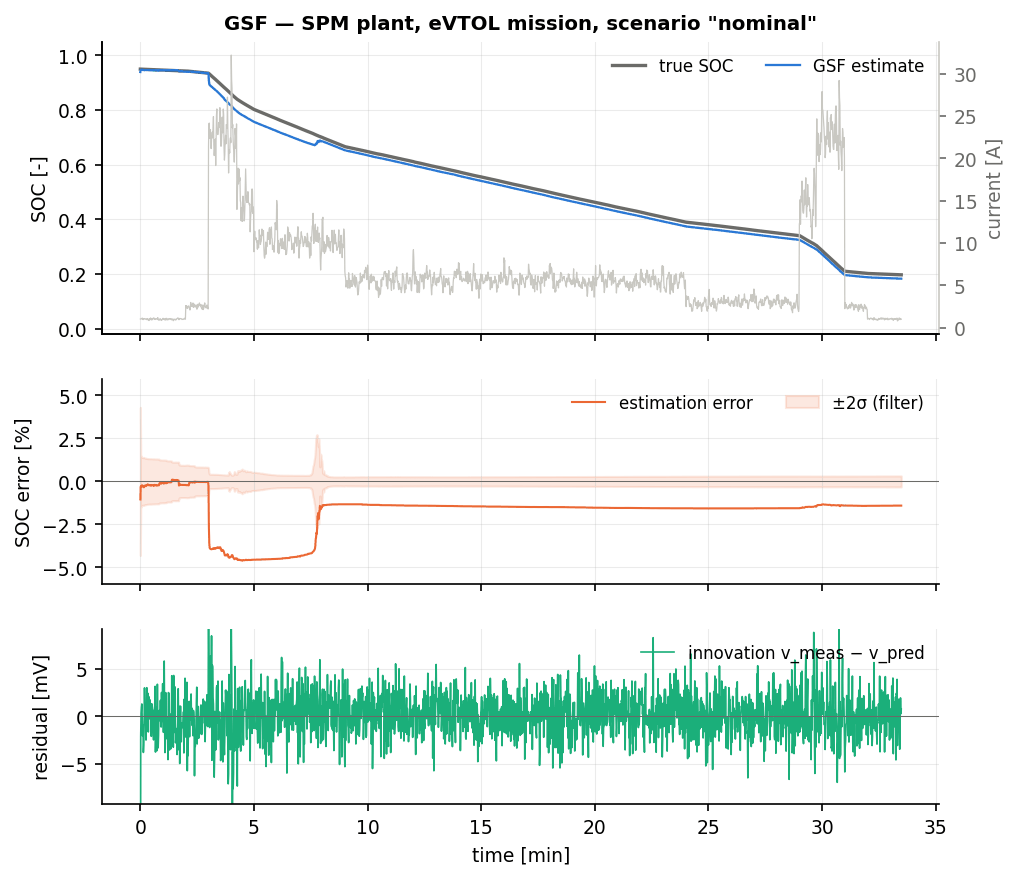
\includegraphics[width=\textwidth]{figures/cellspm_GSF_nominal.png}
\caption{GSF on the electrochemical (SPM) plant, nominal mission: \SI{1.39}{\percent} against
\SI{3.73}{\percent} for the EKF, at \num{3.7} EKFs of cost.}
\end{figure}

\paragraph{Target scenario.}  With a \SI{35}{\percent} initial SOC error the GSF converges
immediately ($t_{\mathrm{conv}} = \SI{0}{\second}$) to $\mathrm{RMSE}_{\mathrm{ss}} =
\SI{0.10}{\percent}$, with a whole-run RMSE of \SI{0.27}{\percent} --- the best initial-error
recovery of the entire family and within a factor of two of the EKF (\SI{0.05}{\percent} /
\SI{0.14}{\percent}) at \num{3.7} times its cost.  The mixture's transient peak is
\SI{7.3}{\percent} against the EKF's \SI{0.62}{\percent}: each component carries only a third of
the prior SOC variance, so its Kalman gain is three times smaller and the first correction is
correspondingly gentler; the weights then shift to the upper component and the estimate catches up
within a few samples.  The honest assessment on the \emph{matched} plant is that the GSF does not
beat a well-tuned EKF at its target scenario, for a reason that belongs to the plant rather than to
the method: over the $\pm3\sigma_{\soc_0}$ interval spanned by the prior, $\ocv(\soc)$ is nearly
affine, so a single linearisation is already adequate and there is no curvature for the mixture to
exploit.  On a chemistry with a pronounced plateau-and-knee OCV (LFP), the same experiment would
look very different.

\paragraph{Where the mixture pays on the ECM plant.}
\begin{itemize}[leftmargin=2em]
  \item \code{combined} --- $\mathrm{RMSE}_{\mathrm{ss}} = \SI{3.33}{\percent}$ with immediate
        convergence, against the EKF's \SI{12.44}{\percent} with \emph{no} convergence at all: a
        factor \num{3.7}, and the difference between a usable and an unusable estimate.  The
        surviving components disagree about SOC, the mixture covariance \eqref{eq:gsf-moments}
        stays honestly large, and the filter keeps listening to the data instead of locking on.
  \item \code{nominal} \SI{0.05}{\percent} and \code{hot} \SI{0.03}{\percent}, both equal to the
        EKF and the best values in this family, at \SI{1.75}{\micro\second}/step.
  \item \code{noise\_step} \SI{0.09}{\percent} and \code{outliers} \SI{0.12}{\percent}, the best of
        the family and better than the EKF (\SI{0.12}{\percent}, \SI{0.21}{\percent}): an outlier
        reduces the weight of all components almost equally and is therefore diluted by the mixture
        rather than absorbed into the state.
  \item \code{sensor\_dropout} \SI{0.10}{\percent}, more than four times better than the EKF's
        \SI{0.46}{\percent}, and \code{preisach} \SI{0.20}{\percent}, equal to the EKF and the best
        of this family by a factor of two --- the corrected hysteresis bias is one of the few
        errors a bank of hypotheses can genuinely arbitrate.
\end{itemize}

\paragraph{Where it is worse than a single EKF.}
\code{aged\_cell} \SI{3.12}{\percent} against \SI{1.52}{\percent} and \code{param\_mismatch}
\SI{2.20}{\percent} against \SI{1.36}{\percent}, with peak errors of \SI{21.7}{\percent} and
\SI{18.2}{\percent}.  The mechanism is the weighting itself: when the \emph{model} is biased, the
component whose SOC offset best compensates the bias wins the likelihood contest, and the mixture
mean follows it.  A single EKF has no such freedom and averages the bias into a smaller error.  This
is the generic hazard of hypothesis-weighted estimators under model error, and it is why
$\delta = 0.5$ (heavily overlapping components, nearly uniform weights) scores \SI{0.77}{\percent}
and \SI{1.31}{\percent} on these two scenarios in the sweep above --- at the cost of failing
\code{combined} exactly as the EKF does.  The trade cannot be tuned away; it has to be addressed by
estimating the parameters (joint or dual estimation) rather than by widening the mixture.

\paragraph{SPM plant.}  Against the electrochemical plant the GSF gives
$\mathrm{RMSE}_{\mathrm{ss}} = \SI{1.39}{\percent}$ on \code{nominal} against the EKF's
\SI{3.73}{\percent} and the UKF's \SI{3.96}{\percent} --- a factor \num{2.7} for \num{3.7} EKFs of
cost, which is the best accuracy-per-flop of any method in this family on that plant.  It also leads
on SPM \code{noise\_step} (\SI{1.21}{\percent} against \SI{3.30}{\percent}), \code{outliers}
(\SI{1.25}{\percent} against \SI{1.99}{\percent}), \code{sensor\_dropout} (\SI{1.85}{\percent}
against \SI{5.31}{\percent}) and \code{hot} (\SI{1.70}{\percent} against \SI{2.16}{\percent}).

The mechanism is a weak form of the one that carries the particle filters.  A bank of three EKFs
displaced along the SOC axis is not a sampling scheme --- each component still makes the linearised
$(\soc, v_2)$ trade-off internally --- but the components make it from \emph{different} SOCs, so the
structured \SI{4}{\milli\volt} residual produces different innovation sequences in each, and the
mixture mean is a likelihood-weighted compromise rather than a single biased trajectory.  That is
enough to halve the EKF's error but not enough to reach the particle filters
(\SIrange{0.62}{0.91}{\percent}), which can place SOC and the RC states anywhere the likelihood
prefers.  The limits show where the model error is largest and most persistent: SPM
\code{current\_bias} \SI{3.86}{\percent} --- still ahead of the EKF's \SI{5.69}{\percent} but
four times behind the particle filters' \SI{0.9}{\percent} --- \code{param\_mismatch}
\SI{3.50}{\percent}, and SPM \code{init\_error} (\SI{3.99}{\percent}) and
\code{cold} (\SI{5.14}{\percent}) never reaching the \SI{2}{\percent} band --- there the same
hypothesis-selection bias that hurts \code{aged\_cell} on the ECM plant is driven continuously by
the structural residual.  Nothing diverges.

\section{Summary}
The Gaussian-sum filter runs a bank of $N_c$ EKFs whose weights are updated by their predictive
likelihoods and whose output is the mixture mean.  It is the cheapest way to keep several
linearisations --- and therefore several hypotheses --- alive: \SI{1.75}{\micro\second}/step,
\SI{9.2}{\kilo\byte}, \num{3.7} EKFs.  On the ECM plant it matches the EKF on \code{nominal}
(\SI{0.05}{\percent}), is the best of this family on \code{noise\_step}, \code{outliers} and
\code{preisach}, converges immediately from a \SI{35}{\percent} initial SOC error, and turns the
EKF's outright failure on \code{combined} (\SI{12.44}{\percent}, no convergence) into
\SI{3.33}{\percent} with immediate convergence.  On the electrochemical plant it halves the EKF's
error (\SI{1.39}{\percent} against \SI{3.73}{\percent}) at a fraction of a particle filter's cost.
Its weakness is the mirror image of its strength: under a biased model the likelihood weighting
selects the component that best compensates the bias, so \code{aged\_cell} and
\code{param\_mismatch} are twice as bad as a single EKF.  Use it whenever the initial SOC is poorly
known, the OCV curve is strongly nonlinear, several fault hypotheses must be carried, or the budget
is a few microseconds; keep the mixture moment-matched, keep the components' spread at
$\delta\approx1$, and do not merge them unless the bank is allowed to grow again.
